\documentclass[a4paper,10pt]{scrartcl}

% Seitenlayout
\usepackage[a4paper,top=1.5cm,right=2.0cm,bottom=2cm,left=2.0cm]{geometry}
\usepackage{fancyhdr}

% Zeichen
\usepackage[ngerman]{babel}
\usepackage[utf8]{inputenc}
\usepackage{amsmath, amsthm, amssymb}
\usepackage{marvosym}
\usepackage[gen]{eurosym}

% Zeichensatz
\usepackage[colorlinks,%
	    citecolor=black,%
	    filecolor=black,%
	    linkcolor=black,%
	    urlcolor=black,%
	    pdftitle = {Mitschrift - CB},%
	    pdfauthor = {Martin Lenders}%
	]{hyperref}
\usepackage{listings}
\usepackage{hyperref}

% Grafik
\usepackage{xcolor}
\usepackage{graphicx}

% Color definitions
\definecolor{lgray}{gray}{0.95}
\definecolor{save}{rgb}{0.498,0,0}
\definecolor{identifier}{rgb}{0,0,0.1}
\definecolor{string}{rgb}{0.192,0,1}
\definecolor{comment}{rgb}{0.25,0.5,0.37}
\definecolor{yellow}{rgb}{1,1,0}
\definecolor{sand}{rgb}{1,1,.75}
\definecolor{red}{rgb}{1,0,0}
\definecolor{melon}{rgb}{1,0.6,.5}
\definecolor{green}{rgb}{0,1,0}
\definecolor{lime}{rgb}{.75,1,.75}
\definecolor{blue}{rgb}{0,0,1}
\definecolor{azure}{rgb}{.75,.75,1}

% Einstellungen für Pakete
\lstset{
	tabsize=8,
	frame=,
	basicstyle=\changefont{pcr}{m}{n},
	emphstyle=\textit,
	numberstyle=\tiny\textsf,
	numbersep=5pt,
	numbers=none,
	keywordstyle=\color{save}\textbf,
	identifierstyle=\color{identifier},
	stringstyle=\color{string},
	showstringspaces=false,
	commentstyle=\color{comment},
	extendedchars=true,
	xleftmargin=1em,
	inputencoding=utf8,
	mathescape=true;
}

\renewcommand{\sectionmark}[1]{\markright{\thesection\ #1}}
\pagestyle{fancy}
\fancyhf{}
\fancyfoot[LE,RO]{\sffamily\thepage}
\fancyhead[LE]{\footnotesize\sffamily\bfseries\leftmark}
\fancyhead[RO]{\footnotesize\sffamily\rightmark} 

% Eigene Befehle
\newcommand{\changefont}[3]{\fontfamily{#1}\fontseries{#2}\fontshape{#3}\selectfont}

% Neudefinitionen
\renewcommand{\sectionmark}[1]{\markright{\thesection\ #1}}

\setlength{\parindent}{0pt}

\title{Lernskript\\\LARGE{}Telematik}
\author{Martin Lenders}

\begin{document}
\maketitle
\tableofcontents
\section{ISO-/OSI-Modell}
% Unterschiede ISO-/OSI <-> TCP/IP
% Netzwerkklassen (PAN, LAN, WAN, ...)

\section{Schicht 1 -- Bitübertragungsschicht}
% synchrone/asynchrone Übertragung
% simplex, duplex, halb-duplex
% Übertragungsmedien
\subsection{Allgemeine Begriffe}
% Overhead, Bandbreite, Throughput, goodput, Paket delivery ratio
% Signal, Data, overhearing, eavesdropping, crosstalk, last mile problem
\subsection{Signalstufen}
\subsubsection{Einheiten}
% bps, baud
\subsubsection{Das Shannon- und Nyquist-Theorem}
\subsection{Codierung}
\subsection{Modulation}
% Constellation diagrams, Frequency Shift Keying

\section{Schicht 2 -- Sicherungsschicht}
\subsection{Allgemeine Begriffe}
% multiplexing, multiple access, packet switching, cell switching, circuit switching
\subsection{Fehlererkennung}
% CRC
\subsection{Fehlerkorrektur}
% FEC / ARQ, Hamming-Code
\subsection{Flusskontrolle}
\subsection{Rahmenerkennung}
% Bit-/Byte-Stuffing, HDLC, PPP, LLC
\subsection{Medium Access}
% ALOHA, CSMA, Kollisionserkennung (CSMA/CD), Kollisionsfreie Protokolle
\subsection{Ethernet}
% IEEE 802.1d, Spanning Tree Protocol, IEEE 802.1q, IEEE 802.2
\subsection{ATM}
% SVC, PVC, VPI, VCI, ATM checksum
\subsection{SDH}
% add drop multiplexer
\subsection{Netzwerk-Infrastruktur}
% Repeater, Hub, Bridges, Switches, Router, Gateway
\subsection{VLANs}

\section{MPLS}
\begin{itemize}
\item   \emph{M}ulti\emph{p}rotocol \emph{L}abel \emph{S}witching
\item   Bündelung von IP und ATM
\item   Weiterleitung von Datenpaketen basiert auf Labels statt Adressen
\item   Unterstützt PPP/Ethernet, ATM, Frame Relay, ...
\item   Unabhängig von Schicht-2- und Schicht-3-Protokollen
\item   Klassifizierung von Paketen beim Betreten einer MPLS-Domäne anhand von
    \begin{itemize}
    \item   Zieladresse, Zielnetzwerk
    \item   QoS
    \item   Anwendung
    \item   VPN
    \item   Multicast-Gruppe
    \item   ...
    \end{itemize}
    $\Rightarrow$ Abbildung zu einer Forward Equivalence Class (FEC)
    \begin{itemize}
    \item   Gruppe von Paketen, die in gleicher Art und Weise über den selben Pfad behandelt werden
    \item   Klassifikation wird nur beim Betreten der MPLS-Domäne im Label codiert
    \end{itemize}
\item   IP-Routing außerhalb einer MPLS-Domäne, Label-Switching innerhalb
        $\Rightarrow$ MPLS-Netzwerk sieht von außen aus wie ein großer IP Router
\item   Komponenten von MPLS:
    \begin{itemize}
    \item   FEC: Forward Equivalence Class
    \item   LSR: Label Switching Router
    \item   LER: Label Edge Router
    \item   LSP: Label Switched Path
    \item   LDP: Label Distribution Protocol
    \end{itemize}
    \begin{center}
    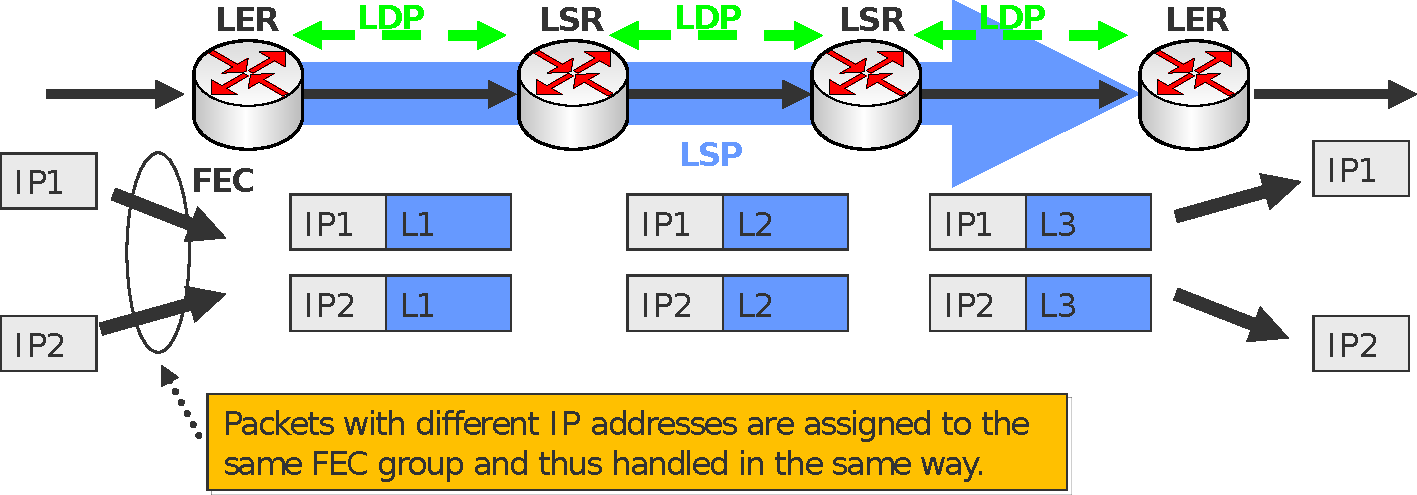
\includegraphics[width=\linewidth]{./MPLS_Components}
    \end{center} 
\item   Explicitly Routed LSP: Netzwerk Provider kann Route genau auswählen $\Rightarrow$ QoS 
\end{itemize}

\subsection{Label}
\begin{itemize}
\item   Label werden aus bestehenden Adressierungselementen gebildet / umbenannt:
    \begin{itemize}
    \item   ATM $\Rightarrow$ VPI/VCI, in jeder Zelle
    \item   Frame Relay $\Rightarrow$ DLCI, in jedem Frame
    \item   ...
    \end{itemize}
\item   Nur lokal gültig
\item   Label können verschiedene Formate haben
\item   Labels können gestapelt werden, nur das höchste wird beachtet, das unterste wird speziell markiert
\item   Generelles Format: 4 Byte
        \begin{itemize}
        \item   20 Bit Label
        \item   3 Bit Experimental (benutzt für QoS)
        \item   1 Bit Bottom Label
        \item   8 Bit TTL
        \end{itemize}
\end{itemize}

\section{Schicht 3 -- Vermittlungsschicht}
\subsection{Allgemeine Begriffe}
% RIR, IXP, Peering, default free zone
\subsection{Aufbau des Internets}
\subsection{Internet Protocol}
% Fragmentierung, Internet Checksum, Multicast (+ Ethernet), Multicast Routing, multihomed hosts
\subsubsection{Adressklassen, Subnetze und CIDR}
\subsubsection{IPv4}
% TOS (DSCP/ECN, historische Nutzung)
\subsubsection{IPv6}
% Privacy Extension, 
\subsubsection{Hilfsprotokolle}
% DHCP, ARP, Stateless Address Auto Configuration (NDP), ICMP, IGMP
\subsection{Routing}
% Routing, Metriken, Verfahren, Tabellen, BGP, Policy Routing, Symmetrische/Asymmetrische Pfade
\subsection{NAT}

\section{Schicht 4 -- Transportschicht}
\subsection{Grundlagen}
% Ports
\subsection{UDP}
\subsection{TCP}
% Fast Retransmit, Fast Recovery, Karn's Algorithmus, Nagle's Algorithmus, Selective and Forward Acknowledgements,
% TCP for networks with high bandwidth-delay product
% Angriffsmöglichkeiten
% Checksum
\subsubsection{Verbindungskontrolle}
\subsubsection{Flusskontrolle}
\subsubsection{Staukontrolle}
% Slow Start
% Congestion Avoidance
% Proactive Congestion Control
% Explicit Congestion Control
\subsection{SCTP}
\subsection{DCCP}

\section{Schicht 5-7 -- Anwendungsprotokolle}
% Client-/Server-Architekturen
\subsection{DNS}
\subsection{E-Mail}
\subsection{WWW}
\subsubsection{HTTP}
\subsubsection{Cookies}
\subsubsection{Proxies}
\subsubsection{HTML}
\subsection{SNMP}
% Public/Private MIB
\subsection{P2P}
% Skalierbarkeit
\subsubsection{DHT}
\subsubsection{Overlay-Topology}
\subsection{Multimedia}
% Multimedia (1. BestEffort, 2. DiffServ, 3. IntServ, SIG, Vorteile, Nachteile)

\end{document}
